\subsection{Open Methods - Chapter 6}

Open methods are deemed open because they are not guaranteed to
converge. The benefit is that if they do converge they converge much
faster than all other methods. That is except for fixed-point
iteration. 

\begin{enumerate}

\item {\bf Simple Fixed-Point Iteration}

Assume for the moment we are trying to solve

\begin{equation}
x^2 - 2x - 3 = 0
\end{equation}

This equation can be re-written intelligently such that

\begin{equation}
x = \frac{x^2-3}{2}
\end{equation}

Notice that the form of this equation is $x=g(x)$ which can actually
be used in an iterative sense. Let us start with an initial guess of
x=0. $g(0) = -3/2$ Thus we set x=-3/2. We then compute $g(-3/2) = -0.375$ and
again we set x=-0.375. When then compute $g(-0.375)$. This process is
repeated over and over again until our change in x is below a certain
threshold. The code for this iteration method can be seen below.

\begin{framed}
\textcolor{blue}{function} xnew = fixed\_point()

x0 = 0;

xnew = g(x0);

xold = x0;

thresh = 1e-2;

\textcolor{blue}{while} abs(xnew - xold) $>$ thresh

~~~~~~xold = xnew;

~~~~~~xnew = (xold\textrm{\^}2-3)/2;

\textcolor{blue}{end}

\end{framed}

The pitfalls of this code are that it takes a large number of
iterations to converge. The example above requires 79,982 iterations. 

\item {\bf Simple Fixed Point Iteration Iterative Algorithm}

The algorithm goes like this:

\begin{enumerate}

\item Convert the Problem into the SFPI form.

\begin{equation}\nonumber
f(x) = 0 \rightarrow x = g(x)
\end{equation}

\item Use the following iterative method

\begin{equation}\nonumber
x_{n+1} = g(x_n)
\end{equation}

\end{enumerate}

\item {\bf The Newton-Raphson Method}

The Newton-Raphson Method is the standard in numerical root
solving. Many additions can be made to the Newton-Raphson Method
however the basic algorithm starts with an initial guess $x_i$,
the function $f(x_i)$, and the derivative of the function
$f'(x_i)$. Then, just like the false position method you create a line
between $f(x_i)$ and zero using a slope equal to $f'(x_i)$ and find
where this line crosses the y-axis. This point is your new point. This
can be seen graphically below and using the equation

\begin{equation}
x_{i+1} = x_i - \frac{f(x_i)}{f'(x_i)}
\end{equation}

\begin{figure}[htb]
  \begin{center}
    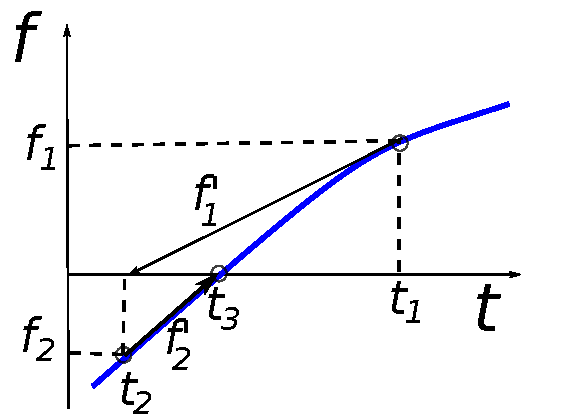
\includegraphics[height=0.45\textwidth,width=0.6\textwidth]{Graphics/NewtonRaphson.pdf}
  \end{center}
\end{figure}

There is an issue associated with the Newton-Raphson technique and
that is convergence. A way to mitigate this issue is by employing a
step size instead of using the entire magnitude of $f'(x_i)$. Thus,
the iterative method becomes

\begin{equation}
x_{i+1} = x_i - \alpha\frac{f(x_i)}{f'(x_i)}
\end{equation}

where $\alpha$ is a step size that is less than 1. It is possible to
have this step size be a variable just like in the bisection method.

\item{\bf The Secant Method (Numerical Version of Newton-Raphson)}

Often times the first derivative of a function is not known. Thus the
Newton-Raphson method cannot be used or rather the first derivative of
the function is replaced with $\tilde{f}$ which is the numerical
derivative of the first derivative.

\item{\bf Error in Newton-Raphson}

Just as with the Trapezoidal rule it is possible to obtain an error
estimate in the Newton-Raphson method. If we write the taylor series
expansion we have

\begin{equation}
f(x_{i+1}) = f(x_i) + f'(x_i)(x_{i+1}-x_i) + f''(\zeta)\frac{(x_{i+1}-x_i)^2}{2!}
\end{equation}

The Newton-Raphson method is derived by setting $f(x_{i+1}) = 0$ and
solving for $x_{i+1}$ assuming that $f'' = 0$.

\begin{equation}
0 = f(x_i) + f'(x_i)(x_{i+1}-x_i)
\end{equation}

Re-arranging the equation above yields the Newton-Raphson method. If
instead we assume that $x_{i+1} = x_r$ or rather in one step we get
the correct answer and let $f'' \neq 0$ we would have

\begin{equation}
0 = f(x_i) + f'(x_i)(x_r-x_i) + f''(\zeta)\frac{(x_r-x_i)^2}{2!}
\end{equation}

since $f(x_r) = 0$. The error in our estimate is then the difference
between the two estimates where $f''=0$ and $f''\neq 0$ we would have


\begin{equation}
0 = f'(x_i)(x_r-x_{i+1}) + f''(\zeta)\frac{(x_r-x_i)^2}{2!}
\end{equation}

Substituting $E_{i+1} = x_r-x_{i+1}$ and assume that $\zeta=x_r$.

\begin{equation}
E_{i+1} = \frac{-f''(x_r)}{2f'(x_r)}E_i^2
\end{equation}

What this means is that if the second derivative of a function is zero
the Newton-Raphson technique will compute the answer in one iteration.

\end{enumerate}


